\documentclass[
a4paper,
10pt,
twoside,
prd,
aps,
nofootinbib,
superscriptaddress,
floatfix,
preprintnumbers,
]{article}


\usepackage{preamble}
\usepackage{titleinfo}

\geometry{ % Set document margins
	top     = 2cm,
	bottom  = 2cm,
	left    = 1cm,
	right   = 1cm
}

\newcommand{\mcols}{1} % Choose number of columns (>= 1)


\bibSetup{refs.bib} % Give references file

% ===== Format headers & footers =====

\pagestyle{fancy}
\fancyhf{}
\fancyhead[LE,RO]{B. Henke}
\fancyhead[LO]{\thetitle\hspace{0.5cm}\textit{PHY803}}
\fancyhead[RE]{\textit{PHY803}\hspace{0.5cm}\thetitle}
\fancyfoot[RE,LO]{\thepage}

\begin{document}
% \tableofcontents
\titleinf
\maketitle
\startmcols

\section{}
\subsection{}
\begin{figure}[H]
    \centering
    \begin{tikzpicture}
    \begin{feynman}
    \vertex (v1);
    \vertex [above left=of v1] (i0)  {$e^-$};
    \vertex [below left=of v1] (i1) {$e^+$};
    \vertex [right=of v1] (v2);
    \vertex [above right=of v2] (f0) {$\mu^+$};
    \vertex [below right=of v2] (f1) {$\mu^-$};
    \diagram* {
    (i0) -- [fermion,momentum = $p_1$] (v1),
    (i1) -- [anti fermion,momentum = $p_2$] (v1),
    (v1) -- [photon, edge label = $\gamma$, momentum' = $q$] (v2),
    (v2) -- [anti fermion,momentum = $p_3$] (f0),
    (v2) -- [fermion,momentum = $p_4$] (f1),
    };
    \end{feynman}
    \end{tikzpicture}
    \caption{This is the $s$-channel diagram for the scattering problem.}
    \label{fig: 4_1}
\end{figure}

\subsection{}
\begin{align}
    M &= (2\pi)^4 \int \left( (\bar{v}(p_2)\gamma^\mu u(p_1)) \left(\frac{ig_e g_{\mu\nu}}{q^2}\right)(\bar{u}(p_4)\gamma^\nu v(p_3)) \delta^4(p_1+p_2-q)\delta^4(q-p_3-p_4) \dd[4]q\right),\\
    &=  \frac{i(2\pi)^4g_e^2}{(p_1+p_2)^2} (\bar{v}(p_2)\gamma^\mu u(p_1))(\bar{u}(p_4)\gamma_\mu v(p_3)) \delta^4(p_1+p_2-p_3-p_4),\\
    \rightarrow
    M &= -\frac{g_e^2}{s} (\bar{v}(p_2)\gamma^\mu u(p_1))(\bar{u}(p_4)\gamma_\mu v(p_3)).
    \label{eq : 1b_ans}
\end{align}

\subsection{}

From \ref{eq : 1b_ans},
\begin{align}
    \abs{M}^2&= \frac{g_e^4}{s^2} (\bar{v}(p_2)\gamma^\mu u(p_1))(\bar{u}(p_4)\gamma_\mu v(p_3)) (\bar{v}(p_2)\gamma^\mu u(p_1))^*(\bar{u}(p_4)\gamma_\mu v(p_3))^*,\\
    \ev{\abs{M}^2} &= \frac{g_e^4}{4s^2} \Tr{\gamma^\mu (\not p_1+m_e)\gamma^\nu (\not p_2-m_e)} \Tr{\gamma_\mu(\not p_3 - m_\mu)\gamma_\nu(\not p_4 + m_\mu)},\\
    &= \frac{4g_e^4}{s^2} \left(\left(p_1^\mu p_2^\nu + p_2^\mu p_1^\nu\right) -g^{\mu\nu} (p_1\cdot p_2) \right) \left(\left(p_{3,\mu} p_{4,\nu} + p_{4,\mu} p_{3,\nu}\right) -g_{\mu\nu} (p_3\cdot p_4)\right),\\
    &=  \frac{4g_e^4}{s^2} \left(\left(p_1^\mu p_2^\nu + p_2^\mu p_1^\nu\right)\left(p_{3,\mu} p_{4,\nu} + p_{4,\mu} p_{3,\nu}\right) + 4 (p_1\cdot p_2)(p_3\cdot p_4)\right.\nonumber\\
    &\qquad - \left. g^{\mu\nu} (p_1\cdot p_2)\left(p_{3,\mu} p_{4,\nu} + p_{4,\mu} p_{3,\nu}\right) - \left(p_1^\mu p_2^\nu + p_2^\mu p_1^\nu\right)g_{\mu\nu} (p_3\cdot p_4) \right),\\
    &= \frac{4g_e^4}{s^2} \left(\left(p_1^\mu p_2^\nu + p_2^\mu p_1^\nu\right)\left(p_{3,\mu} p_{4,\nu} + p_{4,\mu} p_{3,\nu}\right) \right),\\
    &= \frac{4g_e^4}{s^2} \left(2(p_1\cdot p_3)(p_2\cdot p_4) + 2(p_1 \cdot p_4)(p_2 \cdot p_3) \right),\\
    &= \frac{8g_e^4}{s^2} \left((p_1\cdot p_3)(p_2\cdot p_4) + (p_1 \cdot p_4)(p_2 \cdot p_3) \right)
\end{align}

\subsection{}

\begin{align}
    \dv{\sigma}{\Omega} &= \frac{1}{(8\pi)^2} \frac{\ev{\abs{M}^2}}{s}\frac{\abs{\vb{p}_f}}{\abs{\vb{p}_i}},\\
    &= \frac{8g_e^4}{(8\pi)^2 s^2} \frac{((p_1\vdot p_3)(p_2\vdot p_4) + (p_1\vdot p_4)(p_2\vdot p_3))}{s},\\
    &= \frac{g_e^4}{8\pi^2 s^3}\left((p_1\vdot p_3)(p_2\vdot p_4) + (p_1\vdot p_4)(p_2\vdot p_3)\right),\\
    &= \frac{g_e^4}{8\pi^2 s^3} \left((E_e^2 - \abs{\vb{p}_1}\abs{\vb{p}_3}\cos\theta)(E_e^2 - \abs{\vb{p}_2}\abs{\vb{p}_4}\cos\theta) + (E_e^2 + \abs{\vb{p}_1}\abs{\vb{p}_4}\cos\theta)(E_e^2 + \abs{\vb{p}_2}\abs{\vb{p}_3}\cos\theta)\right),\\
    &= \frac{g_e^4}{8\pi^2 s^3} \left((E_e^2 - E_e^2\cos\theta)(E_e^2 - E_e^2\cos\theta) + (E_e^2 + E_e^2\cos\theta)(E_e^2 + E_e^2\cos\theta)\right),\\
    &= \frac{g_e^4}{8\pi^2 s^3} E_e^4\left((1 - \cos\theta)^2+(1 + \cos\theta)^2\right),\\
    &= \boxed{\frac{g_e^4}{512\pi^2 E_e^2} \left(3+\cos2\theta\right).}
\end{align}

\subsection{}

Both go as $1/E_e^2$, however, the interaction we've calculated has a different angular dependence and a magnitude one forth that of the solution given for problem 7.38 in Griffiths.
\begin{figure}[H]
    \centering
    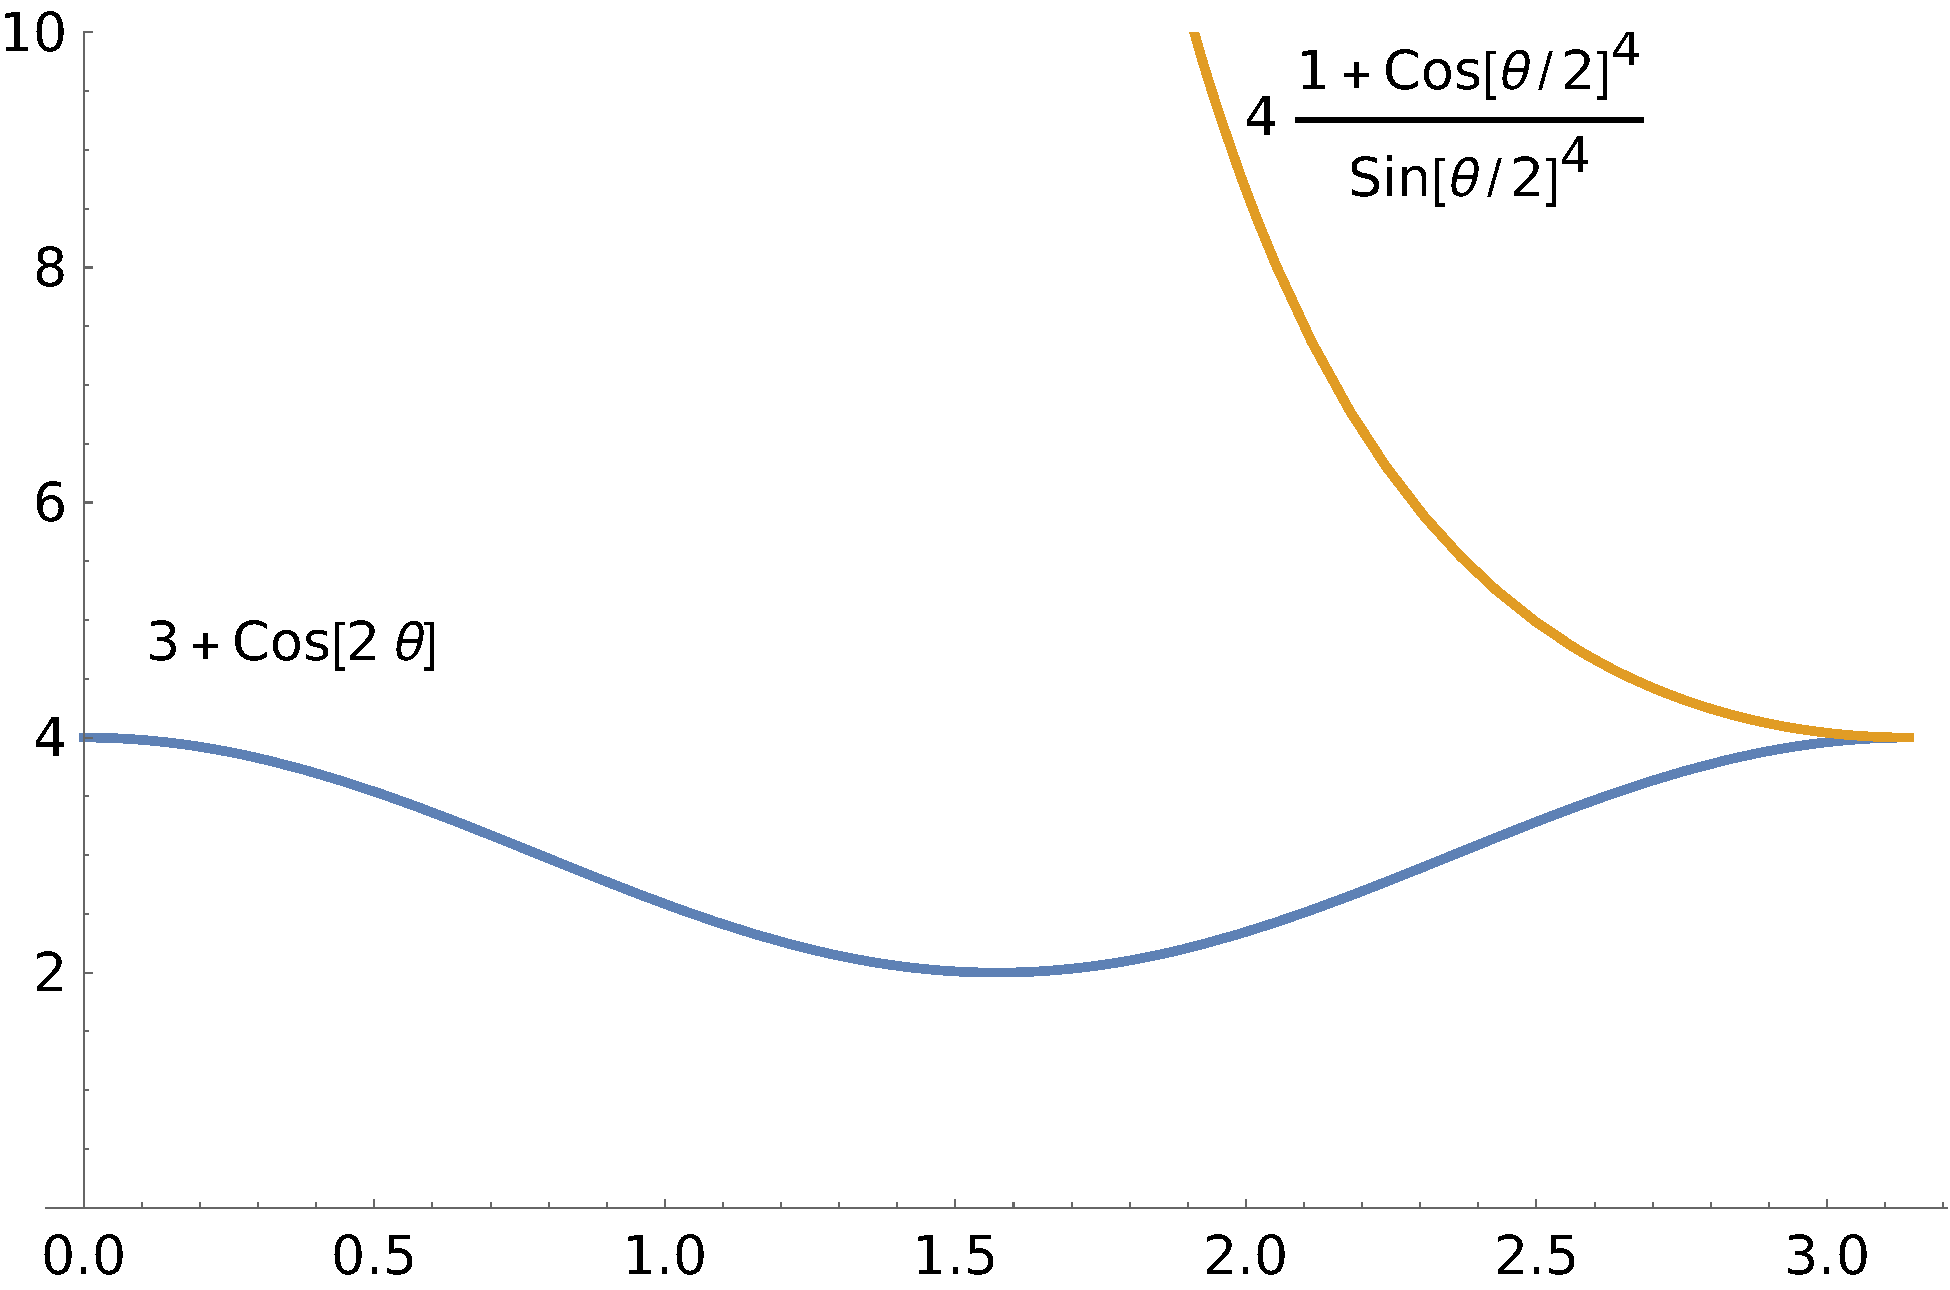
\includegraphics[width=0.5\linewidth]{figures/1e.pdf}
    \caption{%
    This figure shows the angular dependence as found in this problem compared to the angular dependence of problem 7.38 in Griffiths.
    Notice that the dependence found in this problem has an amplitude of one forth that of the dependence in problem 7.38 of Griffiths.
    That is, the two dependencies are equal at $\theta = \pi$, when multiplying one the book's dependence by 4.
    }
    \label{fig:1e_relationship}
\end{figure}


\section{}
\begin{figure}[H]
    \centering
    \begin{tikzpicture}
    \begin{feynman}
    \vertex (v1);
    \vertex [left=of v1] (i0)  {$\gamma$};
    \vertex [above right=of v1] (o0) {$e^-$};
    \vertex [below right=of v1] (o1) {$e^+$};
    \diagram* {
    (i0) -- [        photon,    momentum = $p_1$] (v1),
    (v1) -- [       fermion,    momentum = $p_2$] (o0),
    (v1) -- [  anti fermion,    momentum = $p_3$] (o1),
    };
    \end{feynman}
    \end{tikzpicture}
    \caption{This is the $s$-channel diagram for the decay problem.}
    \label{fig: 4_1}
\end{figure}
\subsection{}
For this instance,
\begin{align}
    M &= i(\bar{u}(p_2) ig_e v(p_3)),\\
    &=  -g_e \bar{u}(p_2) v(p_3).
\end{align}
Thus,
\begin{align}
    \Gamma &= \frac{S\abs{\vb{p}_2}}{8\pi m_\gamma^2} \ev{\abs{M}^2},\\
    &= \frac{\abs{\vb{p}_2}}{8\pi m_\gamma^2} g_e^2 \Tr{(\not p_3-m_e)(\not p_2+m_e)},\\
    &= \frac{g_e^2\abs{\vb{p}_2}}{8\pi m_\gamma^2} (p_2\cdot p_3 - 4m_e^2),\\
    &= \frac{g_e^2\abs{\vb{p}_2}}{8\pi m_\gamma^2} (E_e^2+\vb{p}_2^2 - 4m_e^2),\\
    &= \frac{g_e^2\abs{\vb{p}_2}}{8\pi m_\gamma^2} (2\vb{p}_2^2 - 3m_e^2),\\
    &= \frac{g_e^2\sqrt{m_1^2-4 m_2^2}}{8\pi m_\gamma^3} \left(\frac{1}{4}m_\gamma^2 - m_e^2 - \frac{3}{2}m_e^2\right).
    \label{eq : 2a_ans}
\end{align}
Either I did something wrong (likely) or equation \ref{eq : 2a_ans} simplifies in some way I'm not seeing and is equal to the requested expression.

\subsection{}

The lifetime is $\tau = 1/\Gamma$, so if $m_\gamma = 300$MeV, then $\tau = 6.01\times10^{-22}$s

\nocite{*}
\printbib

\stopmcols


\end{document}

